\part{Hyperparameter Optimization}

\chapter{Stocbio, StocHOAG and the conditioning issue} \label{chp: stoc_cond}
\section{Introduction}
In the field of smooth bilevel optimization, existing deterministic algorithms, based on implicit differentiation of the inner problem, such as HOAG \cite{pedregosa2016hyperparameter} and BA \cite{ghadimi2018approximation}, have been effectively used to solve problems in areas such as hyperparameter optimization. These algorithms, however, exhibit a high per-iteration complexity, in large part due to the inversion of a matrix, that takes place during the implicit differentiation stage. To tackle this issue, stochastic algorithms have been developed. Here, stochasticity is introduced in large part to invert the Hessian in sub-$\mathcal{O}(n^3)$ time. We will be investigating one such algorithm in partiular - stocBio \cite{ji2021bilevel}. This algorithm, albeit having one of the fastest convergence rates among comparable algorithms, requires the tuning of a large number of parameters. Furthermore, stocBio suffers from a sensitivity to the conditioning of the inner problem, much like most other bilevel algorithms. The aim of this report is to investigate a different parameter setup for the algorithm that alleviates this sensitivity.
%\begin{thebibliography}{99}

\subsection{Problem Statement \& Assumptions}
We set up a bilevel problem. For a bounded domain $\mathcal D \subset \mathbb{R}^r$, we wish to find $\lambda \in \mathcal{D}$ and $\hat{x}(\lambda) \in \mathbb{R}^n$, such that
\begin{align} 
&\min_{\lambda \in \mathcal{D}} \mathcal{L}\left(\lambda \right) \triangleq C(\hat{x}(\lambda), \lambda) \label{outer_hoag_neu}\\
&\text { s.t. } \hat{x}(\lambda) =\underset{x \in \mathbb{R}^{n}} \argmin {F(x, \lambda)}. \label{inner_hoag_neu}
\end{align}
\begin{comment}
    We will denote the sampled terms as follows. For i.i.d. samples $\zeta, \xi$, uniformly randomly selected from the given data $\{\zeta_i, \xi_j, i = 1,\hdots, m_1; j = 1,\hdots, m_2 \}$, we have:
\begin{align*}
    \mathbb{E}_{\zeta}[\tilde{F}\left(x, \lambda ; \zeta\right)] &= F\left(x, \lambda\right) \\
    \mathbb{E}_{\xi}[\tilde{C}(x,\lambda,\xi)] &= C(x,\lambda) \\
    %\mathbb{E}_{\theta}[\nabla_\lambda \tilde{C}(x_k,\lambda_k,\theta)] &= \nabla_\lambda \tilde{C}(x_k,\lambda_k) \\
    %\mathbb{E}_{\kappa}[\nabla_{x \lambda}^2 \tilde{F}(x_k,\lambda_k,\kappa)] &= \nabla_{x \lambda}^2 \tilde{F}(x_k,\lambda_k)
\end{align*}

For a function $f:\mathbb{R}^n \xrightarrow[]{} \mathbb{R}$, will denote the conditional expectation $\mathbb{E}_{x_k} [f(x)] = \mathbb{E}[f(x) | x = x_k].$ We introduce some standard assumptions that we will need to tackle this problem.
\end{comment}

% --- Bridge paragraph ---
In many practical applications, the functions $F$ and $C$ are defined as averages over large datasets. 
Computing the exact gradients or Hessians can therefore be prohibitively expensive, especially in high-dimensional settings. 
To alleviate this computational burden, we introduce stochastic approximations, where gradients and function values are computed using randomly sampled subsets of the data. 

Formally, let $\{\zeta_i\}_{i=1}^{m_1}$ and $\{\xi_j\}_{j=1}^{m_2}$ denote the datasets associated with $F$ and $C$, respectively. 
We define the stochastic approximations $\tilde{F}(x, \lambda; \zeta)$ and $\tilde{C}(x, \lambda; \xi)$ as unbiased estimators of $F$ and $C$:
\begin{align*}
    \mathbb{E}_{\zeta}[\tilde{F}\left(x, \lambda ; \zeta\right)] &= F\left(x, \lambda\right), \\
    \mathbb{E}_{\xi}[\tilde{C}(x,\lambda,\xi)] &= C(x,\lambda),
\end{align*}
where $\zeta$ and $\xi$ are drawn uniformly at random from their respective datasets.



\begin{assumption}[Convexity] \label{conv_ass}
    The inner function $F(x, \lambda)$ is $\mu$ strongly-convex w.r.t. $x$.
\end{assumption}

\begin{assumption}[Smoothness] \label{smo_ass}
Let $(x,\lambda) \in \mathbb{R}^{n} \times \mathcal{D}$. The loss function $C(x,\lambda)$ and $F(x,\lambda)$ satisfy the following smoothness assumptions:
\begin{itemize}
    \item The function $C(x,\lambda)$ is $M$-Lipschitz, i.e., for any $(x,\lambda), (x^{\prime},\lambda^{\prime}) \in \mathbb{R}^{n} \times \mathcal{D}$,
$$
\left|C(x,\lambda)-C(x^{\prime},\lambda^{\prime})\right| \leq M\left\|(x,\lambda)-(x^{\prime},\lambda^{\prime})\right\| .
$$
    \item $\nabla C(x,\lambda)$ and $\nabla F(x,\lambda)$ are L-Lipschitz, i.e., for any $(x,\lambda), (x^{\prime},\lambda^{\prime}) \in \mathbb{R}^{n} \times \mathcal{D}$,
$$
\begin{aligned}
\left\|\nabla C(x,\lambda)-\nabla C(x^{\prime},\lambda^{\prime})\right\| & \leq L\left\|(x,\lambda)-(x^{\prime},\lambda^{\prime})\right\|, \\
\left\|\nabla F(x,\lambda)-\nabla F(x^{\prime},\lambda^{\prime})\right\| & \leq L\left\|(x,\lambda)-(x^{\prime},\lambda^{\prime})\right\| .
\end{aligned}
$$
\end{itemize}
For the stochastic case, the same assumptions hold for $C(x,\lambda ; \xi)$ and $F(x,\lambda, \zeta)$ for any given $\xi$ and $\zeta$.
\end{assumption}

An immediate consequence of the previous assumption are bounds on the variances of various sampled gradients:
\begin{proposition}[Bounded variance of $\nabla \tilde{C}, \nabla_{x\lambda}^2 \tilde{F},\nabla_{xx}^2 \tilde{F}$. Lemma 1 in \cite{ji2021bilevel}] \label{boun_var}
    Suppose, Assumption \ref{smo_ass} holds. Then for any $x,\lambda,\zeta$,
    \begin{align*}
        &\mathbb{E}_\zeta \|\nabla \tilde{C}(x,\lambda,\zeta) - \nabla C(x,\lambda)\|^2 \leq M^2 \\
        &\mathbb{E}_\zeta \|\nabla_{x\lambda}^2 \tilde{F}(x,\lambda,\zeta) - \nabla_{x\lambda}^2 F(x,\lambda)\|^2 \leq L^2 \\
        &\mathbb{E}_\zeta \|\nabla_{xx}^2 \tilde{F}(x,\lambda,\zeta) - \nabla_{xx}^2 F(x,\lambda)\|^2 \leq L^2 
    \end{align*}
\end{proposition}

\begin{comment}
    \begin{assumption}[Partial Lipschitz Smoothness] \label{pls_ass}
Let $z = (x,\lambda) \in \mathbb{R}^{n} \times \mathcal{D}$. Suppose the derivatives $\nabla_{x\lambda} F(z)$ and $\nabla_x^2 F(z)$ are $\tau$ - and $\rho$ - Lipschitz, i.e.,
- For any $z, z^{\prime},\left\|\nabla_{x\lambda} F(z)-\nabla_{x\lambda} F(z^{\prime})\right\| \leq \tau\left\|z-z^{\prime}\right\|$.
- For any $z, z^{\prime},\left\|\nabla_x^2 F(z)-\nabla_x^2 F\left(z^{\prime}\right)\right\| \leq \rho\left\|z-z^{\prime}\right\|$.
For the stochastic case, the same assumptions hold for $\nabla_{x\lambda} F(z; \zeta)$ and $\nabla_x^2 F(z ; \zeta)$ for any $\zeta$.
\end{assumption}

\subsection{stocBio and stoc-HOAG}
We begin by introducing the algorithm introduced by Ji et al. that can be used to tackle problem (\ref{outer_hoag_neu}-\ref{inner_hoag_neu}) \cite{ji2021bilevel}. Firstly, we define some of the relevant parameters:
\begin{itemize}
        \item $S$ - the number of samples in every inner SGD step
        \item $D$ - The number of SGD iterations required every time the inner problem is solved.
        \item $D_g$ - the number of samples of $\nabla_{x\lambda} \tilde{F}$ (for every approximate hypergradient).
        \item $D_f$ - The number of samples of $\nabla_x \tilde{C}$ (for every approximate hypergradient).
        \item $\mathcal{S}_{\nabla_\lambda C}$ - the number of samples of $\nabla_{\lambda} \tilde{C}$ (for every approximate hypergradient).
        \item $B$ - The base number of samples of $\nabla_{xx} \tilde{F}$ for the neumann series (\ref{HIA_stocBio}), where the number of samples at the $Q+1-j$-th step of the subroutine is $BQ(1-\eta\mu)^{j-1}.$
    \end{itemize}
Note that the parameters for stocBio are set up in a global manner - at any point during the runtime these are fixed. The Neumann series and its sampling will be explained in section \ref{neumann_series}. The algorithm is described in \ref{alg:stocbio}.
\end{comment}

% --- reformat

\begin{assumption}[Partial Lipschitz Smoothness] \label{pls_ass}
Let $z = (x,\lambda) \in \mathbb{R}^{n} \times \mathcal{D}$. Suppose the derivatives $\nabla_{x\lambda} F(z)$ and $\nabla_x^2 F(z)$ satisfy the following Lipschitz conditions:
\begin{itemize}
    \item For any $z, z^{\prime}$, $\left\|\nabla_{x\lambda} F(z)-\nabla_{x\lambda} F(z^{\prime})\right\| \leq \tau\left\|z-z^{\prime}\right\|$.
    \item For any $z, z^{\prime}$, $\left\|\nabla_x^2 F(z)-\nabla_x^2 F\left(z^{\prime}\right)\right\| \leq \rho\left\|z-z^{\prime}\right\|$.
\end{itemize}
For the stochastic case, the same assumptions hold for $\nabla_{x\lambda} F(z; \zeta)$ and $\nabla_x^2 F(z ; \zeta)$ for any $\zeta$.
\end{assumption}

\subsection{stocBio and stoc-HOAG}
We begin by introducing the algorithm introduced by Ji et al. that can be used to tackle problem (\ref{outer_hoag_neu}-\ref{inner_hoag_neu}) \cite{ji2021bilevel}. Firstly, we define some of the relevant parameters:
\begin{itemize}
    \item $S$: number of samples in every inner SGD step.
    \item $D$: number of SGD iterations required each time the inner problem is solved.
    \item $D_g$: number of samples of $\nabla_{x\lambda} \tilde{F}$ for each approximate hypergradient.
    \item $D_f$: number of samples of $\nabla_x \tilde{C}$ for each approximate hypergradient.
    \item $\mathcal{S}_{\nabla_\lambda C}$: number of samples of $\nabla_{\lambda} \tilde{C}$ for each approximate hypergradient.
    \item $B$: base number of samples of $\nabla_{xx} \tilde{F}$ for the Neumann series (\ref{HIA_stocBio}), where the number of samples at the $(Q+1-j)$-th step of the subroutine is $BQ(1-\eta\mu)^{j-1}$.
\end{itemize}
Note that the parameters for stocBio are set up in a global manner - at any point during the runtime these are fixed. The Neumann series and its sampling will be explained in section \ref{neumann_series}. The algorithm is described in \ref{alg:stocbio}.



\begin{algorithm}[]
\caption{stocBio \cite{ji2021bilevel}}
\label{alg:stocbio}
\DontPrintSemicolon
\KwIn{Outer stepsize $\nu_k$, Neumann length $Q_k$, parameter $\eta$, inner steps $T_k$}
\For{$k = 1, 2, \dots$}{
    Sample batches $D_f$, $\mathcal{S}_{\nabla_\lambda C}$, $D_g$, $\mathcal{B}_j$\;
    Perform $T_k$ steps of SGD on the inner problem with stepsize $\alpha$, yielding $x_k$\;
    Compute Neumann vector:
    \[
    v_Q = \eta \sum_{q=-1}^{Q_k-1} \prod_{j=Q_k - q}^{Q_k} \left(I - \eta \nabla_{xx}^2 \tilde{F}(x_k, \lambda_k; \mathcal{B}_j)\right) \nabla_x \tilde{C}(x_k, \lambda_k, D_f)
    \]
    Compute stochastic gradient:
    \[
    \widehat{\nabla} \mathcal{L}(\lambda_k) = \nabla_\lambda \tilde{C}(x_k, \lambda_k, \mathcal{S}_{\nabla_\lambda C}) - \left( \nabla_{x \lambda}^2 \tilde{F}(x_k, \lambda_k, D_g) \right)^\top v_Q
    \]
    Update hyperparameters:
    \[
    \lambda_{k+1} = \lambda_k - \nu_k \widehat{\nabla} \mathcal{L}(\lambda_k)
    \]
}
\end{algorithm}


The authors also provide theoretical convergence guarantees for this algorithm.
\begin{theorem}[Theorem 3 in \cite{ji2021bilevel}] \label{thm3}
    Suppose assumptions \ref{conv_ass}-\ref{pls_ass} hold. Let $L_{\mathcal{L}(\lambda_k)} = L + \frac{2L^2 + \tau M^2}{\mu} + \frac{\rho L M + L^3 + \tau M L}{\mu^2} + \frac{\rho L^2 M}{\mu^3} = \mathcal{O}(1/\mu^3)$, choose the outer stepsize $\beta$ as $\frac{1}{4 L_\Phi} = \mathcal{O}(\mu^3), \eta < 1/L$, number of inner steps $D \geq \mathcal{O}(\frac{1}{\mu} \log{\frac{1}{\mu}})$. Then
    \[\frac{1}{K} \sum_{k=0}^{K-1} \mathbb{E} \|\nabla \mathcal{L}(\lambda_k)\|^2 \leq \mathcal{O}\left( \frac{L_{\mathcal{L}}}{K} + \frac{L^2(1-\eta \mu)^2Q}{\mu^2} + \frac{L^5 \sigma^2}{\mu^5 S} + \frac{L^2}{\mu^2 D_g} + \frac{L^2}{\mu^2 D_f} + \frac{L^2}{
    \mu^2 B} \right).\]
    
\end{theorem}
Of note here is that, for small $\mu$, the above is bounded as $\mathcal{O}(1/\mu^5)$. As mentioned previously, our aim will be to change the parameter choices in such a manner, that convergence will be less sensitive to an ill-conditioned problem. For this purpose, we will allow the parameters to change with the outer iteration. As such, we relabel them accordingly


\begin{itemize}
        \item $T_k$ - the number of SGD steps to solve the inner problem at the $k-$th outer iteration.
        \item $|\mathcal{S}_{\nabla_{x\lambda} F,k}|$ - the number of samples of $\nabla_{x\lambda} \tilde{F}$ for $k-$th approximate hypergradient.
        \item $|\mathcal{S}_{\nabla_x C,k}|$ - The number of samples of $\nabla_x \tilde{C}$ for $k-$th approximate hypergradient.
        \item $|\mathcal{S}_{\nabla_\lambda C,k}|$ - the number of samples of $\nabla_\lambda \tilde{C}$ for $k-$th approximate hypergradient.
        \item $B_k$ - The base number of samples of $\nabla_{xx} \tilde{F}$ for the Neumann series (\ref{HIA_stocBio}) at $k$-th outer iteration, where the number of samples at the $Q+1-j$-th step of the subroutine is $B_k(1-\eta\mu)^{j-1}$ (for $k-$th approximate hypergradient).
        \item $Q_k$ - Number of Neumann series steps at $k$-th outer iteration.
    \end{itemize}

\begin{algorithm}[]
\caption{Stochastic HOAG}
\label{alg:hoag}
\DontPrintSemicolon
\KwIn{Outer stepsize $\nu_k$, Neumann length $Q_k$, parameter $\eta$, smoothness $\mu$}
\For{$k = 1, 2, \dots$}{
    Sample batches $\mathcal{S}_{\nabla_x C,k}$, $\mathcal{S}_{\nabla_\lambda C,k}$, $\mathcal{S}_{\nabla_{x\lambda} F,k}$, and $\mathcal{B}_j$\;
    Perform $T_k$ steps of SGD on the inner problem with stepsize $\frac{1}{\mu t}$ to obtain $x_k$\;
    Compute Neumann vector:
    \[
    v_Q = \eta \sum_{q=-1}^{Q_k-1} \prod_{j=Q_k - q}^{Q_k} \left(I - \eta \nabla_{xx}^2 \tilde{F}(x_k, \lambda_k; \mathcal{B}_j)\right) \nabla_x \tilde{C}(x_k, \lambda_k, \mathcal{S}_{\nabla_x C,k})
    \]
    Compute stochastic gradient:
    \[
    \widehat{\nabla} \mathcal{L}(\lambda_k) = \nabla_\lambda \tilde{C}(x_k, \lambda_k, \mathcal{S}_{\nabla_\lambda C,k}) - \left( \nabla_{x \lambda}^2 \tilde{F}(x_k, \lambda_k, \mathcal{S}_{\nabla_{x\lambda} F,k}) \right)^\top v_Q
    \]
    Update hyperparameters:
    \[
    \lambda_{k+1} = \lambda_k - \nu_k \widehat{\nabla} \mathcal{L}(\lambda_k)
    \]
}
\end{algorithm}


\section{Main Results}
\subsection{The Neumann Series} \label{neumann_series}
Before we proceed with the convergence analysis of Algorithm \ref{alg:hoag}, let us introduce the Neumann series used for inverting the Hessian, alongside some useful results related to it. As per HOAG, we can obtain the exact hypergradient of the outer problem as
\begin{equation} \label{exact_hyper}
    \nabla\mathcal{L}(\lambda_k) = \nabla_\lambda {C}(\hat{x}(\lambda_k),\lambda_k) - \nabla_{x \lambda}^2 {F}(\hat{x}(\lambda_k),\lambda_k)^\top \left[\nabla_{xx} {F}(\hat{x}(\lambda_k),\lambda_k) \right]^{-1} \nabla_x {C}(\hat{x}(\lambda_k),\lambda_k).
\end{equation}
However, finding the inverse $\left[\nabla_{xx} {F}(\hat{x}(\lambda_k),\lambda_k) \right]^{-1}$ can be costly, and so we consider an approximation for this term. To be more precise, consider the following:

\begin{lemma}[Neumann Series] \label{neumannlem}
For non-singular $A \in \mathbb{R}^{n \times n}$,
\begin{equation} \label{neumann} 
    A^{-1} = \sum^{\infty}_{i=0} (I-A)^i, \quad A \succ 0, \|A\| < 1.
\end{equation}
\end{lemma}
Define, for i.i.d. samples $\xi_0, \zeta_j$, for $j=1,\hdots,Q$,
\begin{equation} \label{HIA_stocBio}
    v_Q= \eta \sum_{q=-1}^{Q-1} \prod_{j=Q-q}^Q\left(I- \eta \nabla_{xx}^2 \tilde{F}\left(x_k, \lambda_k ; \zeta_j\right)\right) v_0, \quad v_0 = \nabla_x \tilde{C}(x_k,\lambda_k,\xi_0),
\end{equation}
where we assume $\prod_{j=Q+1}^Q (\cdot) = I$. Choose $\eta$, such that $\|I- \eta \nabla_{xx}^2 \tilde{F}\left(x_k, \lambda_k ; \zeta_j\right)\| \leq (1-\eta\mu) < 1$. From this, with (\ref{neumann}) we get
\[\mathbb{E}[v_Q] = \eta \sum_{i=0}^{Q} \left[I - \eta\nabla_{xx}^2 F \left(x_k, \lambda_k\right)\right]^i\nabla_x C(x_k,\lambda_k) \approx \left[\nabla_x^2 F\left(x_k, \lambda_k\right)\right]^{-1} \nabla_x C\left(x_k, \lambda_k\right).\]
%As such, denote $\mathbb{E}[v_\infty] = \left[\nabla_x^2 F\left(x_k, \lambda_k\right)\right]^{-1} \nabla_x C\left(x_k, \lambda_k\right) $. 
With this in mind, and the fact that it is not generally feasible to solve the inner problem to full precision, instead of (\ref{exact_hyper}), we use the `approximate hypergradient' in line 3 of our algorithm:
\begin{equation} \label{hat_nabla_def}
                \widehat{\nabla}\mathcal{L}(\lambda_k) = \nabla_\lambda \tilde{C}(x_k,\lambda_k,\mathcal{S}_{\nabla_\lambda C}) - \nabla_{x \lambda}^2 \tilde{F}(x_k,\lambda_k,\mathcal{S}_{\nabla_{x\lambda} F})^\top v_Q.
            \end{equation}
As you will see later, the convergence analysis of our proposed algorithm is directly related to the analytic results regarding $v_Q$. We will provide these now. To begin, we  provide an expectation bound on a $Q-$length Neumann series.
\begin{proposition}[Bound on $\|\mathbb{E}v_Q\|$] \label{evq_bnd}
    Suppose Assumptions \ref{conv_ass}, \ref{smo_ass} hold. Then 
    \[\|\mathbb{E}v_Q\| \leq \frac{M}{\mu}(1-(1-\eta\mu)^{Q+1})\]
\end{proposition}
The variance of the $Q$-long Neumann expansion can be controlled by the sampling of $\nabla_{xx}^2 F$ and $\nabla_x C$ as follows:
\begin{proposition}[Bound on $\mathrm{Var}(v_Q)$] \label{varvq_better}
Suppose Assumptions \ref{conv_ass}, \ref{smo_ass} and \ref{nablaFxl_bnd} hold. Denote the condition number as $\kappa = \frac{L}{\mu}$. Choose $\eta$, such that $\eta \mu < 1.$ Let $|\mathcal{B}_{Q-1+j}| = B(1-\eta\mu)^{j-1}$. Then we have that
    %\[\mathrm{Var}(v_Q) = \mathbb{E}\|v_Q - \mathbb{E}(v_Q)\|^2 \leq \frac{2\eta^3M^2L^2}{\mu}\left(\frac{1 - (1-\eta\mu)^{2Q+2}}{1-(1-\eta\mu)^2} - (1-\eta\mu)^2\frac{1 - (1-\eta\mu)^{3Q+3}}{1-(1-\eta\mu)^3}\right) + 2 \eta^2M^2 \frac{1-(1-\eta\mu)^{2Q}}{1-(1-\eta\mu)^2}.\]
    \[\mathrm{Var}(v_Q) = \mathbb{E}\|v_Q - \mathbb{E}(v_Q)\|^2 \leq   \frac{2 \eta^2M^2 \kappa^2 }{B(1-\eta\mu)} + \frac{2 \eta M^2}{|\mathcal{S}_{\nabla_x C}| (2 - \eta \mu)\mu}.\]
    Furthermore, if in (\ref{HIA_stocBio}) we set $v_0 = \nabla_x C(x_k,\lambda_k)$, then we have
    \[\mathrm{Var}(v_Q) \leq   \frac{\eta^2M^2 \kappa^2 }{B(1-\eta\mu)}.\]
%where $\mathcal{S}_{\nabla_x C}$ refers to the samples for $\nabla_x C(x_k,\lambda_k)$.
\end{proposition}

We now state the bias and variance results for the approximate hypergradient $\widehat{\nabla} \mathcal{L}$. For the bias, we provide the result of Lemma 7 in \cite{ji2021bilevel}:
\begin{proposition}[Bound on $\|\mathbb{E}_{\lambda_k} \widehat{\nabla} \mathcal{L}(\lambda_k) - \nabla \mathcal{L}(\lambda_k)\|.$ Lemma 7 of \cite{ji2021bilevel}] \label{nabla_hat_nabla_bnd}
Suppose Assumptions \ref{conv_ass}, \ref{smo_ass}, \ref{pls_ass} hold. Then we have that 
\[\|\mathbb{E}_{\lambda_k} \widehat{\nabla} \mathcal{L}(\lambda_k) - \nabla \mathcal{L}(\lambda_k)\|^2 \leq 2\left(L + \frac{L^2}{\mu} + \frac{M\tau}{\mu} + \frac{LM\rho}{\mu^2} \right)^2 \|\hat{x}(\lambda_k) - x_k\|^2 + 2 \frac{L^2M^2(1-\eta \mu)^{2Q}}{\mu^2}.\]
\end{proposition}

Similarly, we derive a bound for the variance of $\widetilde{\nabla} \mathcal{L}$:
\begin{proposition}[Bound on $\mathrm{Var}(\widehat{\nabla} \mathcal{L})$] \label{bound_nabla_hat}
Suppose Assumptions \ref{conv_ass}, \ref{smo_ass} and \ref{nablaFxl_bnd} hold. Choose $\eta$, such that $\eta \mu < 1.$ Denote the condition number as $\kappa = \frac{L}{\mu}$. Let $|\mathcal{B}_{Q-1+j}| = B(1-\eta\mu)^{j-1}$. Then the variance of the approximate hypergradient satisfies
\[\mathrm{Var}(\widehat{\nabla} \mathcal{L}(\lambda_k)) = \mathbb{E}\|\widehat{\nabla} \mathcal{L}(\lambda_k) - \mathbb{E}\widehat{\nabla} \mathcal{L}(\lambda_k)\|^2 \leq\]
\[\frac{M^2}{|\mathcal{S}_{\nabla_\lambda C,k}|} 
+ 2 \frac{L^2 M^2}{\mu^2|\mathcal{S}_{\nabla_{x\lambda} F,k}|} \, 
+ 4E^2\eta^2 M^2 \left( \tfrac{\kappa^2}{B (2 - \eta \mu)^2} 
+ \tfrac{1}{|\mathcal{S}_{\nabla_x C,k}|(2\eta \mu - \eta^2 \mu^2)} \right).
\]
\begin{comment}
    \[2\eta^2M^2\left(\frac{\kappa^2}{B (2 - \eta \mu)^2} + \frac{1}{|\mathcal{S}_{\nabla_{x} C,k}|(2\eta \mu - \eta^2 \mu^2)} \right)\left(\frac{L^2}{|\mathcal{S}_{\nabla_{x\lambda} F,k}|} + E^2\right)  +  \frac{\kappa^2M^2}{|\mathcal{S}_{\nabla_{x\lambda} F,k}|}+ \frac{M^2}{|\mathcal{S}_{\nabla_{\lambda} C,k}|}.\]
Furthermore, if in (\ref{HIA_stocBio}) we set $v_0 = \nabla_x C(x_k,\lambda_k)$, then we have
    \[Var(\widehat{\nabla} \mathcal{L}) \leq \eta^2M^2\frac{\kappa^2}{B (2 - \eta \mu)^2} \left(\frac{L^2}{|\mathcal{S}_{\nabla_{x\lambda} F,k}|} + E^2\right)  +  \frac{\kappa^2M^2}{|\mathcal{S}_{\nabla_{x\lambda} F,k}|}+ \frac{M^2}{|\mathcal{S}_{\nabla_{\lambda} C,k}|}.\]
\end{comment}


\begin{comment}
    \begin{align}
\mathrm{Var}(\widehat{\nabla}\mathcal{L})
&\le \frac{M^2}{|\mathcal{S}_{\nabla_{\lambda} C,k}|}
+ \eta^2 M^2\Bigg[
  \Big(\tfrac{8L^2}{|\mathcal{S}_{\nabla_{x\lambda} F,k}|}+4E^2\Big)\frac{\kappa^2}{B(2-\eta\mu)^2} \notag \\[4pt]
&\hspace{3cm}
  + \Big(\tfrac{8L^2}{|\mathcal{S}_{\nabla_{x\lambda} F,k}|}+4E^2\Big)\frac{1}{|\mathcal{S}_{\nabla_x C,k}|(2\eta\mu-\eta^2\mu^2)}
\Bigg]
+ \frac{4L^2M^2}{|\mathcal{S}_{\nabla_{x\lambda} F,k}|\mu^2}.
\end{align}
\end{comment}
    
\end{proposition}


\subsection{Convergence Proof}
Before we proceed to the proof of the convergence, we still need to characterize the smoothness properties of the hypergradient $\nabla \mathcal{L}.$ For this we use the result by Ghadimi \& Wang, 2018 \cite{ghadimi2018approximation}:
\begin{lemma}[$\nabla \mathcal{L}$ is Lipschitz in $\lambda$] \label{nab_lip}
Suppose Assumptions (\ref{conv_ass}), (\ref{smo_ass}) and (\ref{pls_ass}) hold. Then we have, for any $\lambda_1, \lambda_2 \in \mathbb{R}^r$:
\[\|\nabla \mathcal{L}(\lambda_1) - \nabla \mathcal{L}(\lambda_2)\| \leq L_{\mathcal{L}} \|\lambda_1 - \lambda_2\|,\]
where the constant $L_{\mathcal{L}}$ is given by
\[L_{\mathcal{L}} = L + \frac{2L^2 + \tau M^2}{\mu} + \frac{\rho L M + L^3 + \tau M L}{\mu^2} + \frac{\rho L^2 M}{\mu^3}.\]
\end{lemma}
Additionally, we introduce two new assumptions.
\begin{assumption}[Bounded Gradient] \label{nablaFxl_bnd}
    Assume that the partial gradient $\nabla_{x\lambda}^2 F$ is bounded in norm, i.e. $\|\nabla_{x\lambda}^2 F\| \leq E$.
\end{assumption}

\begin{assumption}[Lower bound on objective] \label{inf_ass}
    The sequence of iterates $\left\{\lambda_k\right\}$ is contained in an open set over which $\mathcal{L}$ is bounded below by a scalar $\mathcal{L}_{\text {inf }}$.
\end{assumption}

We now provide a convergence proof for Algorithm \ref{alg:hoag}.
\begin{comment}
\begin{theorem}[Global Convergence] \label{hoag_thm_glcv}

Suppose Assumptions \ref{conv_ass}, \ref{smo_ass}, \ref{pls_ass}, \ref{nablaFxl_bnd} and \ref{inf_ass} hold.
In Algorithm \ref{alg:hoag}, assume that the outer stepsize is chosen as $\nu_k = \frac{1}{2L_\mathcal{L}}$. Suppose $\eta$ is chosen, such that $\eta \mu <1.$Let $\zeta > 0 $ be some small positive number. Choose $Q_k = \frac{r}{2}\log{k^{1+\zeta}}$, where $r > \frac{1}{-\log(1-\eta\mu)}$. Assume also, that $\lambda_k \in \mathcal{D}$ for all $k>0$.
If we choose
\begin{equation}\label{params_conv}
    T_k = \mathcal{O}(k^{1+\zeta}), B_k = |\mathcal{S}_{\nabla_x C,k}| = |\mathcal{S}_{\nabla_{x\lambda} F,k}| = |\mathcal{S}_{\nabla_\lambda C,k}| =\mathcal{O}(k^{1 +\zeta}),
\end{equation}
then we have
\[\min_{k \leq K} \mathbb{E}\|\nabla \mathcal{L}(\lambda_k)\|^2 \xrightarrow[]{K \to \infty} 0\]
 and the above converges at a rate
\[\mathcal{O} \left(\frac{\ln{K}}{K} \right).\]
\end{theorem}
\end{comment}
\begin{theorem}[Global Convergence] \label{hoag_thm_glcv}

Suppose Assumptions \ref{conv_ass}, \ref{smo_ass}, \ref{pls_ass}, \ref{nablaFxl_bnd} and \ref{inf_ass} hold.
In Algorithm \ref{alg:hoag}, assume that the outer stepsize is chosen as $\nu_k = \frac{1}{2L_\mathcal{L}}$. Suppose $\eta$ is chosen such that $\eta \mu < 1$. Let $\zeta > 0$ be some small positive number. Choose $Q_k = \frac{r}{2}\log{k^{1+\zeta}}$, where $r > \frac{1}{-\log(1-\eta\mu)}$. Assume also that $\lambda_k \in \mathcal{D}$ for all $k>0$.
If we choose
\begin{equation}\label{params_conv}
    T_k = \mathcal{O}(k^{1+\zeta}), \quad 
    B_k = |\mathcal{S}_{\nabla_x C,k}| = |\mathcal{S}_{\nabla_{x\lambda} F,k}| = |\mathcal{S}_{\nabla_\lambda C,k}| = \mathcal{O}(k^{1+\zeta}),
\end{equation}
then there exists a constant $C > 0$, independent of $K$, such that
\begin{equation}
\min_{k \le K} \mathbb{E}\|\nabla \mathcal{L}(\lambda_k)\|^2 \le \frac{C \, \ln K}{K}, \quad \forall K \ge 1.
\end{equation}
In particular, this implies
\[
\min_{k \leq K} \mathbb{E}\|\nabla \mathcal{L}(\lambda_k)\|^2 \xrightarrow[K \to \infty]{} 0.
\]
\end{theorem}

%\begin{proof}

\begin{comment}
    \begin{proof}
An equivalent condition to $\mathcal{L}(\lambda)$ having $L_{\mathcal{L}}$-Lipschitz continuous gradient is that for any $\alpha, \beta \in \mathcal{D}$ \cite{Zhou2018}:
\begin{equation} \label{lipschitz_equiv}
    \mathcal{L}(\beta) \le \mathcal{L}(\alpha) + \nabla \mathcal{L}(\alpha)^\top (\beta - \alpha) + \frac{L_{\mathcal{L}}}{2} \|\beta - \alpha\|^2.
\end{equation}

Substitute $\alpha = \lambda_k$, $\beta = \lambda_{k+1} = \lambda_k - \nu_k \widehat{\nabla}\mathcal{L}(\lambda_k)$:
\[
\mathcal{L}(\lambda_{k+1}) \le \mathcal{L}(\lambda_k) - \nu_k \nabla \mathcal{L}(\lambda_k)^\top \widehat{\nabla} \mathcal{L}(\lambda_k) + \frac{L_{\mathcal{L}} \nu_k^2}{2} \|\widehat{\nabla} \mathcal{L}(\lambda_k)\|^2.
\]

Take expectation conditioned on $\lambda_k$:
%\begin{align*}
%\mathbb{E}_{\lambda_k}[\mathcal{L}(\lambda_{k+1})] &\le \mathcal{L}(\lambda_k) - \nu_k \|\mathbb{E}_{\lambda_k}[\widehat{\nabla}\mathcal{L}(\lambda_k)]\|^2 + \nu_k \|\nabla \mathcal{L}(\lambda_k) - \mathbb{E}_{\lambda_k}[\widehat{\nabla}\mathcal{L}(\lambda_k)]\| \cdot \|\mathbb{E}_{\lambda_k}[\widehat{\nabla}\mathcal{L}(\lambda_k)]\| \\
%&\quad + \frac{L_{\mathcal{L}} \nu_k^2}{2} \mathrm{Var}(\widehat{\nabla} \mathcal{L}(\lambda_k)).
%\end{align*}

\begin{align*}
\mathbb{E}_{\lambda_k}\left[\mathcal{L}(\lambda_{k+1})\right] &\leq \mathcal{L}(\lambda_k) -\nu_k \nabla \mathcal{L}(\lambda_k)^\top \mathbb{E}_{\lambda_k}\left[\widehat{\nabla}\mathcal{L}(\lambda_k)\right] + \frac{L_{\mathcal{L}}\nu_k^2 }{2}\mathbb{E}_{\lambda_k}\left[\left\|\widehat{\nabla}\mathcal{L}(\lambda_k)\right\|^2\right] \\
&= \mathcal{L}(\lambda_k) 
- \nu_k \left( \nabla \mathcal{L}(\lambda_k) 
    - \mathbb{E}_{\lambda_k}\left[ \widehat{\nabla} \mathcal{L}(\lambda_k) \right] \right)^\top 
    \mathbb{E}_{\lambda_k}\left[ \widehat{\nabla} \mathcal{L}(\lambda_k) \right] \\
&\quad 
- \nu_k \left\| \mathbb{E}_{\lambda_k} \left[ \widehat{\nabla} \mathcal{L}(\lambda_k) \right] \right\|^2 
+ \frac{L_{\mathcal{L}} \nu_k^2}{2} 
    \mathbb{E}_{\lambda_k} \left[ \left\| \widehat{\nabla} \mathcal{L}(\lambda_k) \right\|^2 \right] \\
&\leq \mathcal{L}(\lambda_k) 
+ \nu_k \left\| \nabla \mathcal{L}(\lambda_k) 
    - \mathbb{E}_{\lambda_k} \left[ \widehat{\nabla} \mathcal{L}(\lambda_k) \right] \right\| 
    \left\| \mathbb{E}_{\lambda_k} \left[ \widehat{\nabla} \mathcal{L}(\lambda_k) \right] \right\| \\
&\quad 
- \nu_k \left\| \mathbb{E}_{\lambda_k} \left[ \widehat{\nabla} \mathcal{L}(\lambda_k) \right] \right\|^2 
+ \frac{L_{\mathcal{L}} \nu_k^2}{2} 
  \mathbb{E}_{\lambda_k} \left[ \left\| \widehat{\nabla} \mathcal{L}(\lambda_k) \right\|^2 \right]\\
  &= \mathcal{L}(\lambda_k) 
+ \nu_k \left\| \nabla \mathcal{L}(\lambda_k) 
  - \mathbb{E}_{\lambda_k} \left[ \widehat{\nabla} \mathcal{L}(\lambda_k) \right] \right\| 
  \left\| \mathbb{E}_{\lambda_k} \left[ \widehat{\nabla} \mathcal{L}(\lambda_k) \right] \right\| \\
&\quad 
+ \frac{L_{\mathcal{L}} \nu_k^2}{2} 
  \mathrm{Var} \left( \widehat{\nabla} \mathcal{L}(\lambda_k) \right) 
- \left( \nu_k 
  - \frac{L_{\mathcal{L}} \nu_k^2}{2} \right) 
  \left\| \mathbb{E}_{\lambda_k} \widehat{\nabla} \mathcal{L}(\lambda_k) \right\|^2
\end{align*}

We now define the terms bounding bias and variance of the approximate hypergradient:

\[
D_{1,k} = \sqrt{2}\left(L + \frac{L^2}{\mu} + \frac{M\tau}{\mu} + \frac{LM\rho}{\mu^2} \right) \|\hat{x}(\lambda_k) - x_k\|,
\quad 
D_{2,k} = \sqrt{2} \frac{LM(1-\eta \mu)^{Q_k}}{\mu},
\]

\[
D_{3,k} = \frac{M^2}{|\mathcal{S}_{\nabla_\lambda C,k}|} 
+ 2 \frac{L^2 M^2}{\mu^2|\mathcal{S}_{\nabla_{x\lambda} F,k}|} 
+ 4E^2\eta^2 M^2 \left( \frac{\kappa^2}{B_k (2 - \eta \mu)^2} + \frac{1}{|\mathcal{S}_{\nabla_x C,k}| (2\eta \mu - \eta^2 \mu^2)} \right).
\]

Using the bounds from Propositions \ref{nabla_hat_nabla_bnd} and \ref{bound_nabla_hat},
\[
\|\mathbb{E}_{\lambda_k}[\widehat{\nabla} \mathcal{L}(\lambda_k)] - \nabla \mathcal{L}(\lambda_k)\|^2 \le D_{1,k}^2 + D_{2,k}^2, \quad \mathrm{Var}(\widehat{\nabla} \mathcal{L}(\lambda_k)) \le D_{3,k},
\]
we obtain
\begin{equation} \label{totele3_clean}
(\nu_k - L_{\mathcal{L}} \nu_k^2) \|\nabla \mathcal{L}(\lambda_k)\|^2 \le 4 \mathcal{L}(\lambda_k) - 4 \mathbb{E}_{\lambda_k}[\mathcal{L}(\lambda_{k+1})] + 6 \nu_k (D_{1,k}^2 + D_{2,k}^2) + 2 L_{\mathcal{L}} \nu_k^2 D_{3,k}.
\end{equation}

Since $\nu_k = 1/(2 L_\mathcal{L})$, we have $\nu_k - L_{\mathcal{L}} \nu_k^2 = 1/(4 L_\mathcal{L}) > 0$.  

Summing (\ref{totele3_clean}) from $k=1$ to $K$, taking total expectation, and telescoping the first term, we get
\begin{equation} \label{tele_ineq_clean}
\sum_{k=1}^K (\nu_k - L_{\mathcal{L}} \nu_k^2) \mathbb{E}\|\nabla \mathcal{L}(\lambda_k)\|^2 \le 4 \mathcal{L}(\lambda_1) - 4 \mathcal{L}_{\inf} + \sum_{k=1}^K \left( 6 \nu_k \mathbb{E}[D_{1,k}^2] + 6 \nu_k D_{2,k}^2 + 2 L_{\mathcal{L}} \nu_k^2 D_{3,k} \right).
\end{equation}

By our choice of parameters (\ref{params_conv}) and Lemma \ref{sgdmu}, each term in the sum on the right-hand side is $\mathcal{O}(1/k^{1+\zeta})$, so
\[
\sum_{k=1}^K \left( 6 \nu_k \mathbb{E}[D_{1,k}^2] + 6 \nu_k D_{2,k}^2 + 2 L_{\mathcal{L}} \nu_k^2 D_{3,k} \right) = \mathcal{O}(\ln K).
\]

The denominator grows as
\[
\sum_{k=1}^K (\nu_k - L_{\mathcal{L}} \nu_k^2) = K / (4 L_\mathcal{L}) = \mathcal{O}(K).
\]

Hence, the convergence rate follows:
\[
\min_{k \le K} \mathbb{E}\|\nabla \mathcal{L}(\lambda_k)\|^2 \le \frac{\mathcal{O}(\ln K)}{\mathcal{O}(K)} = \mathcal{O}\left(\frac{\ln K}{K}\right),
\]
as claimed.
\end{proof}
\end{comment}




%\begin{comment}
\begin{proof}
    An equivalent condition to $\mathcal{L}(\lambda)$ having $L_{\mathcal{L}}-$Lipschitz continuous gradient is that for any $\alpha,\beta \in \mathcal{D}$ \cite{Zhou2018}:
\begin{equation} \label{lipschitz_equiv}
    \mathcal{L}(\beta) \leq \mathcal{L}(\alpha) + \nabla \mathcal{L}(\alpha)^\top (\beta - \alpha) + \frac{L_{\mathcal{L}}}{2}\|\beta - \alpha\|^2.
\end{equation}
Substituting for $\alpha = \lambda_k, \beta = \lambda_{k+1} = \lambda_k - \nu_k\widehat{\nabla}\mathcal{L}(\lambda_k)$,

\[\mathcal{L}(\lambda_{k+1}) \leq \mathcal{L}(\lambda_k) + \nabla \mathcal{L}(\lambda_k)^\top \left(-\nu_k\widehat{\nabla}\mathcal{L}(\lambda_k)\right) + \frac{L_{\mathcal{L}}}{2}\left\|-\nu_k\widehat{\nabla}\mathcal{L}(\lambda_k)\right\|^2,\]
where $\widehat{\nabla} \mathcal{L}(\lambda_k)$ is the approximate hypergradient of $\mathcal{L}$, evaluated at $\lambda_k$, as defined in step 3 of Algorithm \ref{alg:hoag}. Taking expectation, conditioning on $\lambda_k$,

\begin{align*}
\mathbb{E}_{\lambda_k}\left[\mathcal{L}(\lambda_{k+1})\right] &\leq \mathcal{L}(\lambda_k) -\nu_k \nabla \mathcal{L}(\lambda_k)^\top \mathbb{E}_{\lambda_k}\left[\widehat{\nabla}\mathcal{L}(\lambda_k)\right] + \frac{L_{\mathcal{L}}\nu_k^2 }{2}\mathbb{E}_{\lambda_k}\left[\left\|\widehat{\nabla}\mathcal{L}(\lambda_k)\right\|^2\right] \\
&= \mathcal{L}(\lambda_k) 
- \nu_k \left( \nabla \mathcal{L}(\lambda_k) 
    - \mathbb{E}_{\lambda_k}\left[ \widehat{\nabla} \mathcal{L}(\lambda_k) \right] \right)^\top 
    \mathbb{E}_{\lambda_k}\left[ \widehat{\nabla} \mathcal{L}(\lambda_k) \right] \\
&\quad 
- \nu_k \left\| \mathbb{E}_{\lambda_k} \left[ \widehat{\nabla} \mathcal{L}(\lambda_k) \right] \right\|^2 
+ \frac{L_{\mathcal{L}} \nu_k^2}{2} 
    \mathbb{E}_{\lambda_k} \left[ \left\| \widehat{\nabla} \mathcal{L}(\lambda_k) \right\|^2 \right] \\
&\leq \mathcal{L}(\lambda_k) 
+ \nu_k \left\| \nabla \mathcal{L}(\lambda_k) 
    - \mathbb{E}_{\lambda_k} \left[ \widehat{\nabla} \mathcal{L}(\lambda_k) \right] \right\| 
    \left\| \mathbb{E}_{\lambda_k} \left[ \widehat{\nabla} \mathcal{L}(\lambda_k) \right] \right\| \\
&\quad 
- \nu_k \left\| \mathbb{E}_{\lambda_k} \left[ \widehat{\nabla} \mathcal{L}(\lambda_k) \right] \right\|^2 
+ \frac{L_{\mathcal{L}} \nu_k^2}{2} 
  \mathbb{E}_{\lambda_k} \left[ \left\| \widehat{\nabla} \mathcal{L}(\lambda_k) \right\|^2 \right]\\
  &= \mathcal{L}(\lambda_k) 
+ \nu_k \left\| \nabla \mathcal{L}(\lambda_k) 
  - \mathbb{E}_{\lambda_k} \left[ \widehat{\nabla} \mathcal{L}(\lambda_k) \right] \right\| 
  \left\| \mathbb{E}_{\lambda_k} \left[ \widehat{\nabla} \mathcal{L}(\lambda_k) \right] \right\| \\
&\quad 
+ \frac{L_{\mathcal{L}} \nu_k^2}{2} 
  \mathrm{Var} \left( \widehat{\nabla} \mathcal{L}(\lambda_k) \right) 
- \left( \nu_k 
  - \frac{L_{\mathcal{L}} \nu_k^2}{2} \right) 
  \left\| \mathbb{E}_{\lambda_k} \widehat{\nabla} \mathcal{L}(\lambda_k) \right\|^2
\end{align*}



\begin{equation} \label{Lip_to_sub}
    \leq \mathcal{L}(\lambda_k) + \frac{\nu_k}{2} \left\|\nabla \mathcal{L}(\lambda_k)- \mathbb{E}_{\lambda_k}\left[\widehat{\nabla}\mathcal{L}(\lambda_k)\right]\right\|^2 + \frac{L_{\mathcal{L}}\nu_k^2}{2}\mathrm{Var}(\widehat{\nabla}\mathcal{L}(\lambda_k)) - \left(\frac{\nu_k}{2} - \frac{L_{\mathcal{L}}\nu_k^2}{2}\right) \|\mathbb{E}_{\lambda_k} \widehat{\nabla}\mathcal{L}(\lambda_k)\|^2,
\end{equation}
Denote
\[D_{1,k} = \sqrt{2}\left(L + \frac{L^2}{\mu} + \frac{M\tau}{\mu} + \frac{LM\rho}{\mu^2} \right) \|\hat{x}(\lambda_k) - x_k\|, \quad D_{2,k} = \sqrt{2} \frac{LM(1-\eta \mu)^{Q_k}}{\mu}\]
Recall, that by Proposition \ref{nabla_hat_nabla_bnd}, we have a bound on the bias of $\widehat{\nabla} \mathcal{L}$ as
\begin{equation} \label{T45diff}
    \|\mathbb{E}_{\lambda_k} \widehat{\nabla} \mathcal{L}(\lambda_k) - \nabla \mathcal{L}(\lambda_k)\|^2 \leq D_{1,k}^2  + D_{2,k}^2,
\end{equation}
from which we immediately obtain
\[\|\mathbb{E}_{\lambda_k} \widehat{\nabla} \mathcal{L}(\lambda_k) - \nabla \mathcal{L}(\lambda_k)\| \leq D_{1,k}  + D_{2,k}.\]
By reverse triangle inequality, we have that
\[\left| \|\mathbb{E}_{\lambda_k} \widehat{\nabla} \mathcal{L}(\lambda_k) \| - \|\nabla \mathcal{L}(\lambda_k)\| \right| \leq D_{1,k}+D_{2,k}, \text{ hence } \|\mathbb{E}_{\lambda_k} \widehat{\nabla} \mathcal{L}(\lambda_k) \| \geq \|\nabla \mathcal{L}(\lambda_k)\| -  (D_{1,k}+D_{2,k}).\]
%\begin{equation} \label{Enabhat}
%    \|\mathbb{E}_{\lambda_k} \widehat{\nabla} \mathcal{L}(\lambda_k) \| \leq D_{1,k}+D_{2,k} + \|\nabla \mathcal{L}(\lambda_k)\| \quad \mathrm{and} \quad 
%\end{equation}

Furthermore, using $(a+b)^2 \leq 2a^2 + 2b^2$, we obtain the following lower bound for $\|\mathbb{E}_{\lambda_k} \widehat{\nabla} \mathcal{L}(\lambda_k) \|^2$:
\begin{equation} \label{Enabhatsq_rev}
    \|\mathbb{E}_{\lambda_k} \widehat{\nabla} \mathcal{L}(\lambda_k) \|^2 \geq \frac{\|\nabla \mathcal{L}(\lambda_k)\|^2 - 4D_{1,k}^2 -4D_{2,k}^2}{2}.
\end{equation}
\\Finally, by proposition \ref{bound_nabla_hat}, we have the variance bound 

\begin{align}
\mathrm{Var}\left( \widehat{\nabla} \mathcal{L}(\lambda_k) \right) 
&\frac{M^2}{|\mathcal{S}_{\nabla_\lambda C,k}|} 
+ 2 \frac{L^2 M^2}{\mu^2|\mathcal{S}_{\nabla_{x\lambda} F,k}|} \,  \notag \\
&\quad + 4E^2\eta^2 M^2 \left( \tfrac{\kappa^2}{B (2 - \eta \mu)^2} 
+ \tfrac{1}{|\mathcal{S}_{\nabla_x C,k}|(2\eta \mu - \eta^2 \mu^2)} \right)
\triangleq D_{3,k}.
\label{varbndthm}
\end{align}


%Set $M_1 = T_{45}^2 + 2T_{45}$, $M_2 = 2T_{45} + 1$. 
Substituting (\ref{T45diff}),(\ref{Enabhatsq_rev}) and (\ref{varbndthm}) into (\ref{Lip_to_sub}), noting that $\mathcal{L}(\lambda) = C(\hat{x}(\lambda),\lambda)$ is $L_\mathcal{L}$-lipschitz and rearranging, we get
\begin{equation} \label{totele3}
    (\nu_k - L_{\mathcal{L}}\nu_k^2)\|\nabla \mathcal{L} (\lambda_k)\|^2 \leq 4\mathcal{L}(\lambda_k) - 4\mathbb{E}_{\lambda_k}\left[\mathcal{L}(\lambda_{k+1})\right]+ 2D_{3,k}\nu_k^2 L_{\mathcal{L}} + 6\nu_k(D_{1,k}^2 + D_{2,k}^2).
\end{equation}
Firstly, note that $\nu_k - L_{\mathcal{L}}\nu_k^2 = \frac{1}{4L_\mathcal{L}} > 0$.
Summing (\ref{totele3}) for $k = 1$ to $\infty$, we get
\[\sum_{k=1}^\infty (\nu_k - L_{\mathcal{L}}\nu_k^2)\|\nabla\mathcal{L}(\lambda_k)\|^2 \leq \sum_{k=1}^\infty \left( 4\mathcal{L}(\lambda_k) - 4\mathbb{E}_{\lambda_k}\left[\mathcal{L}(\lambda_{k+1})\right]\right) + \sum_{k=1}^\infty \left( 2D_{3,k}\nu_k^2 L_{\mathcal{L}} + 6\nu_k(D_{1,k}^2 + D_{2,k}^2) \right).\]
Taking total expectation and telescoping, we get
\begin{equation} \label{tele_ineq}
    \sum_{k=1}^\infty (\nu_k - L_{\mathcal{L}}\nu_k^2)\mathbb{E}\|\nabla\mathcal{L}(\lambda_k)\|^2 \leq  4\mathcal{L}(\lambda_1) - 4\mathcal{L}_{inf} + \sum_{k=1}^\infty \left(2D_{3,k}\nu_k^2 L_{\mathcal{L}} + 6\nu_k\mathbb{E}[D_{1,k}^2] + 6\nu_kD_{2,k}^2\right).
\end{equation}
Recall our choice $\eta_k = \frac{1}{2L_\mathcal{L}}$. From (\ref{params_conv}), Lemma \ref{sgdmu} and by the choice of $Q_k$, we have
$$D_{3,k}\nu_k^2 = \mathcal{O}\left(\frac{1}{k^{1+\zeta}}\right), \quad \nu_k\mathbb{E}[D_{1,k}^2] = \mathcal{O}\left(\frac{1}{k^{1+\zeta}} \right), \quad \nu_k D_{2,k}^2 = \mathcal{O}\left(\frac{1}{k^{1+\zeta}} \right).$$
Hence, we have that 
\[\sum_{k=1}^\infty \left(2D_{3,k}\nu_k^2 L_{\mathcal{L}} + 6\nu_k\mathbb{E}[D_{1,k}^2] + 6\nu_kD_{2,k}^2\right) = \sum_{k=1}^\infty \mathcal{O}\left(\frac{1}{k^{1+\zeta}}\right) < \infty.\]
Thus, the right-hand side of the inequality (\ref{tele_ineq}) is finite, and so
\begin{equation} \label{weighted_sum}
    \sum_{k=1}^\infty (\nu_k - L_{\mathcal{L}}\nu_k^2)\mathbb{E}\|\nabla\mathcal{L}(\lambda_k)\|^2 < \infty
\end{equation}
Furthermore, from (\ref{weighted_sum}), we get that
\[\min_{k \leq K} \mathbb{E}\|\nabla \mathcal{L}(\lambda_k)\|^2 \leq \frac{\sum_{k=1}^K (\nu_k - L_{\mathcal{L}}\nu_k^2)\mathbb{E}\|\nabla\mathcal{L}(\lambda_k)\|^2}{\sum_{k=1}^K (\nu_k - L_{\mathcal{L}}\nu_k^2)} \xrightarrow[]{K \to \infty} 0\]
%\[\liminf_{k \to \infty} \mathbb{E}\|\nabla\mathcal{L}(\lambda_k)\|^2 = 0.\]
Finally, recalling our choice of stepsize $\nu_k = \frac{1}{2L_\mathcal{L}}$, and other parameters in (\ref{params_conv}), we obtain
\[\sum_{k=1}^K (\nu_k - L_{\mathcal{L}}\nu_k^2) = \mathcal{O} \left(K \right), \quad \sum_{k=1}^K (\nu_k - L_{\mathcal{L}}\nu_k^2)\|\nabla\mathcal{L}(\lambda_k)\|^2 = \mathcal{O} \left(\frac{1}{\zeta} - \frac{1}{\zeta K^\zeta} \right) \xrightarrow[]{\zeta \to 0} \mathcal{O}\left(\ln{K} \right),\]
giving us a convergence rate of
\[\mathcal{O} \left(\frac{\ln{K}}{K} \right).\]
\end{proof}
%\end{comment}



%\end{proof}

\section{Comparison with stocBio}
In the following sections we will compare our setup to that of Ji et. al. In light of that, let us recall the motivations for this comparison. The two major points that we address are:
\begin{itemize}
    \item Relaxed parameter choices - we want to relax the parameter choices in such a way that we still maintain similar rates of convergence, while improving upon the sensitivity to the inner problem condition.
    \item Modularity - we want to devise an algorithm with comparable convergence guarantees to stocBio, where the theoretical base allows for inner problem solver other than SGD.
\end{itemize}
\begin{comment}
    We will begin by comparing the assumptions of the two methods. Stochastic HOAG shares the assumptions of stocBio, with the exception of \ref{nablaFxl_bnd}, the boundedness of $\nabla^2_{x \lambda} F$. %While the two methods both assume bounds on $\|x_k - \hat{x}(\lambda_k)\|$, in our case we only require that this is bounded in expectation.
stocBio and Stochastic HOAG share mostly the same parameters, but their choices vary between the two methods. Firstly, for our bound on $\mathbb{E}\|x_k - \hat{x}(\lambda_k)\|$ to be a summable sequence, it is sufficient to choose the number of inner loop steps as $\sqrt{k} + \zeta$, for small $\zeta > 0$. In comparison, stocBio has a fixed number of inner-loop steps, dependent on the smoothness and convexity parameters. Regarding the Neumann series subroutine, while $Q_k$ was chosen in both cases as $\mathcal{O}(\log{k})$, the choice for the batch size of the samples of $\nabla^2_{xx} F$ was different. We allowed for a constant batch size, while in the case of stocBio,  this was taken as $BQ(1-\eta \mu)^{j-1}$, for some large constant $B$. That is, the batch size starts large initially, but decays exponentially as we progress through the inversion subroutine. Finally, the sampling for $\nabla_x C$ was also with constant batch sizes in our case, but was done as $\mathcal{O}(\log{k})$ in the case of stocBio. By Theorem 3 of stocBio, we have the following convergence result:
\[\frac{1}{K} \sum_{k=0}^{K-1} \mathbb{E}\|\nabla\mathcal{L}(\lambda_k)\|^2 = \mathcal{O}\left( 1/K \right).\]
In theory, stocBio has a much faster convergence rate, but the choice of such parameters as the batches for stochastic gradient and hessians was less trivial.
\end{comment}

\subsection{Gradient Complexities and the Conditioning Problem} \label{mu_comp}
Before we begin with any comparisons, let us define the following:
\begin{definition}[$\epsilon$-accurate stationary point]
    For an output of the algorithm $\bar{\lambda}$, we say that $\bar{\lambda}$ is an $\epsilon$-accurate stationary point of $\mathcal{L}(\lambda)$ if $\mathbb{E}\|\nabla\mathcal{L}(\bar{\lambda})\| \leq \epsilon$.
\end{definition}

In the paper by Ji et al. the following assumption is made, akin to our assumption \ref{conv_ass}.

\begin{assumption}[Convexity]
    The inner function $F(x, \lambda)$ is $\mu$ strongly-convex w.r.t. $x$. For the stochastic setting, the same assumption holds for $\tilde{F}(x, \lambda ; \zeta)$.
\end{assumption}

However, this assumption doesn't generally hold if we expect $\mu$ to be large enough. For example, if $F$ is the ridge-regularized least-squares loss,
\[F(x,\lambda) = \frac{1}{2}\|Ax-b\|_2^2 + \frac{e^\lambda}{2}\|x\|_2^2,\]
then the lower bound on the convexity of $F$ is given by the minimum eigenvalue $\mu_0$ of
\[A^T A + e^\lambda \mathrm{Id}\]
and, assuming $A^T A$ is not full-rank,
\[\min_{\lambda \in \mathbb{R}} \mu_0 = 0.\]
In practice, this bound is never achieved, as $\lambda$ is on a bounded domain, but $\mu_0$ still may be very small. In light of that, let us recall the convergence bound, obtained in the same paper:

\begin{theorem}[Theorem 3 in \cite{ji2021bilevel}] \label{thm3}
    Suppose, that Assumptions \ref{conv_ass}-\ref{pls_ass} hold. Let $L_{\mathcal{L}(\lambda_k)} = L + \frac{2L^2 + \tau M^2}{\mu} + \frac{\rho L M + L^3 + \tau M L}{\mu^2} + \frac{\rho L^2 M}{\mu^3} = \mathcal{O}(1/\mu^3)$, choose the outer stepsize $\beta$ as $\frac{1}{4 L_\Phi} = \mathcal{O}(\mu^3), \eta < 1/L$, number of inner steps $D \geq \mathcal{O}(\frac{1}{\mu} \log{\frac{1}{\mu}})$. Then
    \[\frac{1}{K} \sum_{k=0}^{K-1} \mathbb{E} \|\nabla \mathcal{L} (\lambda_k)\|^2 \leq \mathcal{O}\left( \frac{L_{\mathcal{L}}}{K} + \frac{L^2(1-\eta \mu)^2Q}{\mu^2} + \frac{L^5 \sigma^2}{\mu^5 S} + \frac{L^2}{\mu^2 D_g} + \frac{L^2}{\mu^2 D_f} + \frac{L^2}{
    \mu^2 B} \right),\]
    where
    \begin{itemize}
        \item $S$ - the number of samples in every inner SGD step
        \item $D$ - The number of SGD iterations required every time the inner problem is solved.
        \item $D_g$ - the number of samples of $\nabla_{x\lambda} \tilde{F}$ (for every approximate hypergradient).
        \item $D_f$ - The number of samples of $\nabla_x \tilde{C}$ (for every approximate hypergradient).
        \item $\mathcal{S}_{\nabla_\lambda C}$ - the number of samples of $\nabla_{\lambda} \tilde{C}$ (for every approximate hypergradient).
        \item $B$ - The base number of samples of $\nabla_{xx} \tilde{F}$ for the neumann series (\ref{HIA_stocBio}), where the number of samples at the $Q+1-j$-th step of the subroutine is $BQ(1-\eta\mu)^{j-1}.$
    \end{itemize}
\end{theorem}
As mentioned previously, the left-hand-side above is bounded at the very least as $\mathcal{O}(1 / \mu^5)$. Additionally, to reach an $\epsilon$-close stationary point, the gradient complexities of the inner and outer problems, respectively, must satisfy
\[GC(C,\epsilon) = KDS = \mathcal{O}(\mu^{-9} \epsilon^{-2}), \quad GC(F,\epsilon) = KD_f = \mathcal{O} (\mu^{-5} \epsilon^{-2}). \]
Additionally, the Hessian vector complexity (From the Neumann series subroutine) must satisfy
\[HV(\epsilon) = K \sum_{j=1}^Q B Q(1-\eta \mu)^{j-1} = \mathcal{O}\left(\frac{1}{\mu^6\epsilon^2} \ln \frac{1}{\mu^2\epsilon}\right).\]
Of note is the extreme complexity of the inner problem with respect to its condition $\mu$. Let us inspect whether our parameter choices improve the $\mu$-complexity or the convergence bound sensitivity to $\mu$. Note, that, analogous to Theorem \ref{thm3}, we can derive a similar result for our case, using the consequences of Theorem \ref{hoag_thm_glcv} above. Inspect line \ref{tele_ineq} in our convergence proof. Lower-bounding the left hand side, we obtain
\begin{equation} \label{tele_ineq2}
    \frac{1}{K}\sum_{k=1}^K \mathbb{E}\|\nabla\mathcal{L}(\lambda_k)\|^2 \leq  \frac{L_\mathcal{L}\left(4\mathcal{L}(\lambda_1) - 4\mathcal{L}_{inf}\right)}{K} + \frac{1}{K}\sum_{k=1}^K \left(2D_{3,k}\nu_k^2 L^2_{\mathcal{L}} + 6\nu_kL_\mathcal{L}\mathbb{E}[D_{1,k}^2] + 6\nu_k D_{2,k}^2\right),
\end{equation}
where,
\[D_{1,k} = \sqrt{2}\left(L + \frac{L^2}{\mu} + \frac{M\tau}{\mu} + \frac{LM\rho}{\mu^2} \right) \|\hat{x}(\lambda_k) - x_k\|, \quad D_{2,k} = \sqrt{2} \frac{LM(1-\eta \mu)^{Q_k}}{\mu},\]
%\begin{equation} \label{varbndthm2}
%    D_{3,k} = 2\eta^2M^2\left(\frac{\kappa^2}{B_k (2 - \eta \mu)^2} + \frac{1}{|\mathcal{S}_{\nabla_{x} C,k}|(2\eta \mu - \eta^2 \mu^2)} \right)\left(\frac{L^2}{|\mathcal{S}_{\nabla_{x\lambda} F,k}|} + E^2\right)  +  \frac{\kappa^2M^2}{|\mathcal{S}_{\nabla_{x\lambda} F,k}|}+ \frac{M^2}{|\mathcal{S}_{\nabla_{\lambda} C,k}|}.
%\end{equation}
\begin{equation} \label{varbndthm2}
    D_{3,k} = \frac{M^2}{|\mathcal{S}_{\nabla_\lambda C,k}|} 
+ 2 \frac{L^2 M^2}{\mu^2|\mathcal{S}_{\nabla_{x\lambda} F,k}|} \, 
+ 4E^2\eta^2 M^2 \left( \tfrac{\kappa^2}{B (2 - \eta \mu)^2} 
+ \tfrac{1}{|\mathcal{S}_{\nabla_x C,k}|(2\eta \mu - \eta^2 \mu^2)} \right)
\end{equation}
Note, that $\zeta>0$ in Theorem \ref{hoag_thm_glcv} affects the summation on the RHS of (\ref{tele_ineq2}). If $\zeta$ is large enough, then the sum is bounded by $\mathcal{O}(1/\zeta)$ and doesn't grow with $K$. On the other hand, if $\zeta$ is small, then the smallest upper bound for the sum is $\mathcal{O}(\ln{K})$. Assume that $\zeta$ is large enough, so that the dependence of the RHS of (\ref{tele_ineq2}) on $K$ is as $\mathcal{O}\left( \frac{1}{K} \right)$. Then, to achieve an $\epsilon-$accurate stationary point, we must have at least, that
\[\frac{L_\mathcal{L}}{K} = \epsilon \implies K = \mathcal{O}\left(\frac{1}{\mu^3 \epsilon} \right).\]
We will now provide the complexities for the individual parameters and will finish this section by providing a $\mu$-convergence bound. We begin with the complexities for the individual samples sizes in $D_{3,k}$. Using our choices in (\ref{params_conv}), we obtain the following gradient complexities. The total number of samples for gradients $\nabla_{x}C, \nabla_{x\lambda} F$ and $\nabla_\lambda C$ are
\[\sum_{k=1}^K k^{1+\zeta} = \mathcal{O} \left(K^{2+\zeta} \right) \approx \mathcal{O}\left(\frac{1}{\mu^6\epsilon^2}\right).\]
Coincidentally, this gives us the outer gradient complexity as $GC(F,\epsilon) = \mathcal{O}(\mu^{-6}\epsilon^{-2})$.
%Inspecting the $D_{1,k}$ term in \ref{tele_ineq2}, using Lemma \ref{sgdmu}, we get that $T_k = \mathcal{O}\left(\frac{1}{\mu^3 }k^{1-s+\zeta}\right)$. Thus, the gradient complexity of the inner problem, assuming we conduct single-sample SGD, is
%\[\sum_{k=1}^K T_k = \frac{1}{\mu^3}\sum_{k=1}^{K} k^{1-s+\zeta} = \mathcal{O}(K^{2-s+\zeta}) \approx \mathcal{O} \left(\frac{1}{\mu^6 \epsilon} \frac{1}{(\mu^3 \epsilon)^\frac{1}{1-s}} \right),\]
Regarding the inner problem, we get that $T_k = \mathcal{O}\left(k^{1+\zeta}\right)$. Thus, the inner problem complexity, i.e., the total number of steps of the inner problem, assuming we conduct single-sample SGD, is
\[GC(C,\epsilon) = \sum_{k=1}^K T_k = \sum_{k=1}^{K} k^{1+\zeta} = \mathcal{O}(K^{2+\zeta}) \approx \mathcal{O} \left(\frac{1}{\mu^6 \epsilon^2}\right).\]
Finally, let us inspect the Neumann series. Note, that to achieve an $\epsilon$-accurate point, we must have base samples to grow as $B_k = \mathcal{O} \left( k^{1+\zeta} \right)$. Thus, the Neumann series complexity is
\[HV(\epsilon) = \sum_{k=1}^K \sum_{j=1}^{Q_k} B_k (1-\eta\mu)^{j-1}=\sum_{k=1}^K B_k \frac{1 - \frac{1}{\sqrt{k^{1+\zeta}}}}{\eta\mu} = \mathcal{O}\left(\frac{1}{\mu^7 \epsilon^2} \right).\]
As we see, while the outer gradient complexity and the Hessian-vector complexities have slightly worsened, the gradient complexity of the inner problem has improved by an order of $\mu^3$. Let us now provide a $\mu$-convergence bound. For this purpose, we inspect the three terms $D_{1,k}, D_{2,k}, D_{3,k}$ in (\ref{varbndthm2}). For the sake of simplicity we consider only the case $s=0$. Using Lemma \ref{sgdmu}, we get that $\mathbb{E} [D_{1,k}^2] = \mathcal{O}\left(\frac{1}{\mu^6}\sum_{k=1}^K\frac{1}{T_k}\right) \approx \mathcal{O}\left(\frac{1}{\mu^6}\ln{\frac{1}{\mu}}\right)$. Next, let us inspect $D_{2,k}^2$. Substituting the value of $Q_k$ from Theorem \ref{hoag_thm_glcv}, we get that $D_{2,k}^2 \approx \mathcal{O} \left( \frac{1}{\mu^2} \ln{\frac{1}{\mu}}\right)$. Finally, inspecting the $D_{3,k}$ term, we get that
\[\sum^{K}_{k=1} D_{3,k} = \mathcal{O}\left( \frac{\kappa^2}{B_k (2 - \eta \mu)^2} \right) \approx \mathcal{O}\left( \frac{1}{\mu^4} \ln{\frac{1}{\mu}} \right).\]

As such, bringing $\mathbb{E} [D_{1,k}^2], D_{2,k}^2, D_{3,k}$ into (\ref{tele_ineq2}), we get that the left hand side is bounded by at most $\mathcal{O}\left( \frac{1}{\mu^3} \ln{\left( \frac{1}{\mu} \right)} \right)$. Compared to the parametrisation of Ji et al. we see an improvement at least on the order of $\mu$.

\begin{comment}
    \subsection{Conditioning in a Quadratic Problem}
As we have observed, the bilevel algorithm's performance is poor for non-strongly convex problems. However for a inner problem, quadratic in $x$, such as
\[F(x,\lambda) = \frac{1}{2}\|Ax-b\|_2^2 + \frac{e^\lambda}{2}\|x\|_2^2,\]
we can improve upon this. For a start, we provide a reformulation of Proposition \ref{nabla_hat_nabla_bnd}:
\begin{proposition}[Bound on $\|\mathbb{E}_{\lambda_k} \widehat{\nabla} \mathcal{L}(\lambda_k) - \nabla \mathcal{L}(\lambda_k)\|.$ Lemma 7 of \cite{stocBio}.] \label{nabla_hat_nabla_bnd_v2}
Suppose assumptions \ref{conv_ass}, \ref{smo_ass}, \ref{pls_ass} hold. Assume furthermore, that $F(x,\lambda)$ is quadratic in $x$. Then we have that 
\[\|\mathbb{E}_{\lambda_k} \widehat{\nabla} \mathcal{L}(\lambda_k) - \nabla \mathcal{L}(\lambda_k)\|^2 \leq 2\left(L + \frac{L^2}{\mu} + \frac{M\tau}{\mu}  \right)^2 \|\hat{x}(\lambda_k) - x_k\|^2 + 2 \frac{L^2M^2(1-\eta \mu)^{2Q}}{\mu^2}.\]
\end{proposition}
\begin{proof}
    
\end{proof}
As such, we manage to drop a factor of $\frac{1}{\mu^2}$ from the above bound. The consequences of this change in our case and for stocBio, we present below.
\begin{theorem}[Theorem 3 in \cite{stocBio} (Quadratic Problem)] \label{thm3v2}
    Suppose all of the assumptions in \cite{stocBio} hold. Assume furthermore, that $F(x,\lambda)$ is quadratic in $x$. Let $L_{\mathcal{L}(\lambda_k)} = L + \frac{2L^2 + \tau M^2}{\mu} + \frac{\rho L M + L^3 + \tau M L}{\mu^2} + \frac{\rho L^2 M}{\mu^3} = \mathcal{O}(1/\mu^3)$, choose the outer stepsize $\beta$ as $\frac{1}{4 L_\Phi} = \mathcal{O}(\mu^3), \eta < 1/L$, number of inner steps $D \geq \mathcal{O}(\frac{1}{\mu} \log{\frac{1}{\mu}})$. Then
    \[\frac{1}{K} \sum_{k=0}^{K-1} \mathbb{E} \|\nabla \mathcal{L}\|^2 \leq \mathcal{O}\left( \frac{L_{\mathcal{L}}}{K} + \frac{L^2(1-\eta \mu)^2Q}{\mu^2} + \frac{L^5 \sigma^2}{\mu^3 S} + \frac{L^2}{\mu^2 D_g} + \frac{L^2}{\mu^2 D_f} + \frac{L^2}{
    \mu^2 B} \right),\]
    where
    \begin{itemize}
        \item $S$ - the number of samples in every inner SGD step
        \item $D_g$ - the number of samples of $\nabla_{x\lambda} \tilde{F}$ (for every approximate hypergradient).
        \item $D_f$ - The number of samples of $\nabla_x \tilde{C}$ (for every approximate hypergradient)
        \item $B$ - The base number of samples of $\nabla_{xx} \tilde{F}$ for the neumann series (\ref{HIA_stocBio}), where the number of samples at the $Q+1-j$-th step of the subroutine is $BQ(1-\eta\mu)^{j-1}.$
    \end{itemize}
\end{theorem}

As a consequence, the convergence bound scales as $\mathcal{O}\left(\frac{1}{\mu^3}\right)$. As such, to obtain an $\epsilon$-accurate stationary point, we must choose the inner number of steps (for stocBio) $S = \mathcal{O}(\frac{1}{\mu^3 \epsilon})$, as opposed to $S = \mathcal{O}(\frac{1}{\mu^5 \epsilon})$ previously. From this, we get that the gradient complexity of the inner problem is now $\mathcal{O}(\frac{1}{\mu^7 \epsilon^2})$. Analogously, in our case, the $D_{1,k}$ term in line \ref{tele_ineq2} is now
\[D_{1,k} = \sqrt{2}\left(L + \frac{L^2}{\mu} + \frac{M\tau}{\mu} \right) \|\hat{x}(\lambda_k) - x_k\|,\]
and so the $\mu$-complexity of the $\mathbb{E}D_{1,k}^2$ term (for $s=0$) is now $\mathcal{O}\left(\frac{1}{\mu^4} \ln{\left( \frac{1}{\mu} \right)} \right)$. In turn, once again comparing the $\mathbb{E} [D_{1,k}^2], D_{2,k}^2, D_{3,k}$ terms within (\ref{tele_ineq2}), we get that the $\mu$-complexity of the right-hand-side of (\ref{tele_ineq2}) is now $\mathcal{O}\left(\frac{1}{\mu} \ln{\left( \frac{1}{\mu} \right)} \right)$.
\end{comment}

\subsection{ISGD for Hessian Inverse}
As the aim of this chapter was to present a robust algorithm for smooth bilevel optimization, it was natural that we also consider the Hessian inverse subroutine. The common approach with a stochastic Neumann series, as in \ref{HIA_stocBio}, requires setting a stepsize $\eta$. However, if set too large, then the subroutine may diverge. For this reason, we introduce an alternative implicit Euler subroutine for inverting the Hessian $\nabla_{xx} F$. Let us formalize this. Note that the neumann series (\ref{HIA_stocBio}) can be rewritten as 
\begin{equation} \label{neumann_step}
    v_{Q_{t+1}} = v_{Q_{t}} - \eta \nabla_{xx}^2 \tilde{F}(x_k,\lambda_k,\zeta_t) v_{Q_{t}} + \eta v_{Q_0}, \quad \text{ with } v_{Q_0} = \nabla_x C
\end{equation}
Let us ignore the $\nabla_x C$ term for now and set $v_{Q_0} = \eta Id$. Additionally, assume $\nabla_{xx}^2 \tilde{F}(x_k,\lambda_k,\zeta_t) = \nabla_{xx}^2 F(x_k,\lambda_k)$. Now, consider the matrix ODE
\begin{equation} \label{neumann_ode}
    \dot{v}_{Q_{t}} = Id - \nabla_{xx}^2 F v_{Q_{t}} \triangleq G(v_{Q_{t}}).
\end{equation}
We have that (\ref{neumann_step}) is a step of the Euler method for (\ref{neumann_ode}) with stepsize $\eta$. This motivates us to consider the implicit Euler discretization of (\ref{neumann_ode}). That is, we now write
\[v_{Q_{t+1}} = v_{Q_{t}} + \eta G(v_{Q_{t+1}}) = v_{Q_{t}} + \eta Id - \eta \nabla_{xx}^2 F v_{Q_{t+1}}.\]
Thus,
\[v_{Q_{t+1}} = (Id + \eta \nabla_{xx}^2 F)^{-1}(v_{Q_{t}} + \eta Id);\]
In light of our problem, we consider the update
\begin{equation} \label{impl_neu}
    v_{Q_{t+1}} = (Id + \eta \nabla_{xx}^2 \tilde{F}_t)^{-1}(v_{Q_{t}} + \eta Id)
\end{equation}
where, assuming $\nabla_{xx}^2 \tilde{F}_t$ is low-rank, we can leverage the Woodbury matrix identity to invert the system. The update (\ref{impl_neu}) is a step of implicit stochastic gradient descent. 



\section{Numerics}
We did not conduct an empirical study of the effect of conditioning on convergence, but we did compare the performance of Stocbio and Stoc-HOAG on the same problem. We generate a random gaussian train matrix $A \in \mathbb{R}^{10 \times 20}$ and a sparse solution vector $x_0 \in \mathbb{R}^{10}$. We construct the data vector $y = Ax_0 + err$, where $err \in \mathbb{R}^{10}$ is some small gaussian error vector. Then the problem we will be trying to tackle is
\begin{align} 
&\min_{\lambda \in \mathcal{D}} \mathcal{L}\left(\lambda \right) \triangleq \|\hat{x}(\lambda) - x_0\|_2^2 \label{outer_hoag_test}\\
&\text { s.t. } \hat{x}(\lambda) =\underset{x \in \mathbb{R}^{n}} \argmin \frac{1}{2}\|A x - y\|_2^2 + \frac{e^\lambda +\mu_0}{2}\|x\|_2^2. \label{inner_hoag_test},
\end{align}

where $\mu_0 > 0$ is a global strong-convexity parameter, that ensures the inner problem is always at least $\mu_0$-strongly convex. Obviously, in a practical setting having this parameter is not realistic, but in our case, when the optimal value $\lambda$ is almost always close to $0$, it allows us to gauge the effect of strong convexity on convergence. We will compare Stocbio to a few variations of Stoc-HOAG. The difference between these comes down to how we tackle the inner problem and the Hessian inverse. We will compare 
\begin{enumerate}
    \item Stoc-HOAG with SGD for inner problem and $v_Q$ computed via Neumann series;
    \item Stoc-HOAG with conjugate gradient descent for inner problem and $v_Q$ computed via Neumann series;
    \item Stoc-HOAG with SGD for inner problem and $v_Q$ updated via ISGD.
\end{enumerate}

We run for $\mu_0 = 1$, 20000 outer iterations. The results are presented in Figure \ref{fig:stoc_bio_hoag} below. The Stoc-HOAG algorithms all feature a comparable $\mathcal{O}\left( 1/K \right)$ convergence to Stocbio in this toy problem, suggesting that we can obtain even tighter guarantees that of Theorem \ref{hoag_thm_glcv}.
\begin{figure}
    \centering
    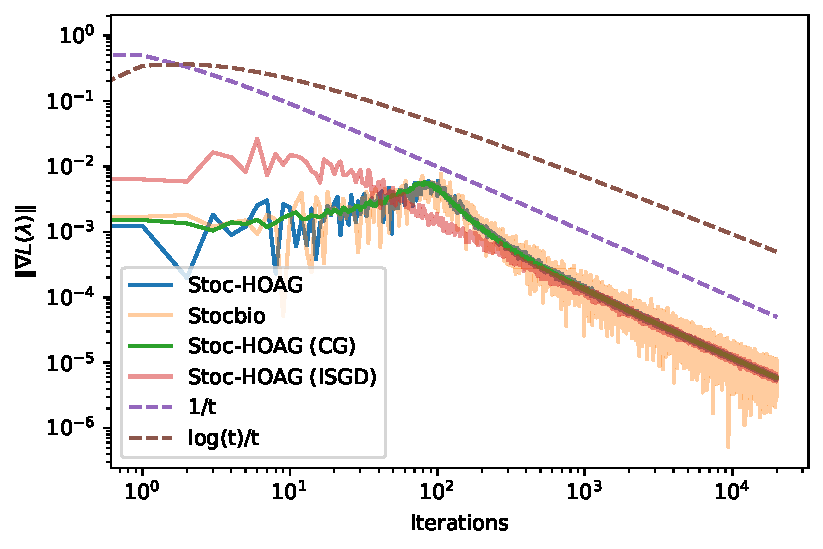
\includegraphics[width=0.5\linewidth]{IMG/stochoag/a_run_of_STHOAG_grad.pdf}
    \caption{Convergence comparison of Stocbio and Stoc-HOAG}
    \label{fig:stoc_bio_hoag}
\end{figure}

The code for reproducing numerics in this section is available at the \href{https://github.com/icheltso/thesis/tree/main/thesis\_stoc\_hoag}{thesis\_stoc\_hoag} folder of the Github repository.

\section{Conclusion}
The stocBio algorithm is one of the more recent approaches to stochastic bilevel optimisation. However, as with many other algorithms, designed to tackle bilevel problems, it suffers from a high sensitivity to the strong-convexity parameter $\mu$ of the inner level problem. In this chapter we introduce a reparametrisation for the algorithm that make it more robust in this regard, providing comparable practical convergence and improving complexity with regards to $\mu$.